\documentclass[]{scrartcl}
\usepackage[spanish]{babel}

\decimalpoint
%opening
\usepackage{xcolor}
\usepackage{mathtools}
\usepackage{graphicx}
\usepackage{enumitem}
\usepackage{hyperref}
\newcommand{\tt}[1]{\texttt{#1}}
\definecolor{bitacora}{HTML}{217821}
\newcommand{\that}[0]{\texttt{THAT~}}

\usepackage{siunitx}
\sisetup{output-decimal-marker = {.}}

\title{Práctica 3 de control: control robusto de un sistema de primer orden usando un controlador PI\\}


\author{Leonardo Bermeo}

\begin{document}
	
	\maketitle
%
%
%


\section{Control PI de un sistema de primer orden} 

Ahora vamos a usar el THAT para diseñar, simular e  implementar un controlador PI para controlar un sistema de primer orden. 

La planta que vamos a controlar tiene función de transferencia

 \[G(s)=\dfrac{5}{s+0.5}.\]
Y usaremos un control PI de dos grados de libertad, como se muestra en la figura~\ref{fig:controlPI-1gdl}.
\begin{figure}[h!]
	\centering
	
\includegraphics[width=0.8\linewidth]{figuras/control_PI_2gdl.pdf}
	\caption{Control PI para la planta $\frac{5}{s+0.5}$}
	\label{fig:controlPI-1gdl}
\end{figure}
\newpage

\subsubsection*{Pasos}

\begin{enumerate}
	\item Diseñe en un controlador PI de dos grados de libertad para satisfacer los siguientes requerimientos de diseño:
	\begin{itemize}
		\item $SP \approx 10\%$
		\item $t_{ee} \approx 0.7\text{ s} $
	\end{itemize}

	
	\item Dibuje correctamente el diagrama de computación analógica con bloques del \that que  implementa el diagrama de la figura~\ref{fig:controlPI-1gdl}. Tenga en cuenta las inversiones de signo que producen los sumadores e integradores. Use el mínimo número de bloques.
	

		% Tenga en cuenta que la planta $G(s)$ ya tiene a $y$ y $-y$.}
	
	%Para ello proponemos el diagrama de computador analógico de la figura~\ref{fig:pi_compan}.
		%
%	\begin{figure}[h!]
%		\centering
%		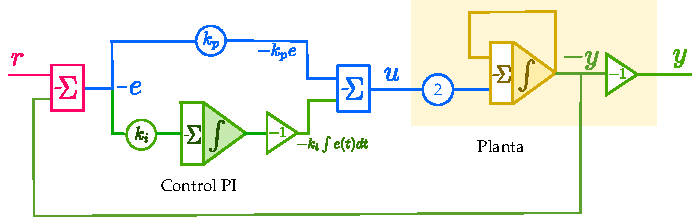
\includegraphics[width=.8\textwidth]{figuras/PI_comp_analog.pdf}
%		\caption{Implementación de un coeficiente mayor a la unidad.}
%		\label{fig:pi_compan}.
%	\end{figure}
	
 %Implemente el sistema de lazo cerrado de la figura~\ref{fig:pi_compan}.

  \item Construya el generador de onda cuadrada de la práctica 2 y úselo como entrada de referencia $r$. Sincronice esta señal en el canal 1 del osciloscopio. 
 

 \item Implemente su diagrama del sistema de control  en el \that. Ajuste los valores de $k_p$ y $k_i$ del controlador en el THAT (es posible que tenga que usar multiplicador $\times$ 10 en los bloques de suma o integración) y verifique la respuesta obtenida.  
 
  \item Registre la respuesta obtenida en el osciloscopio para el controlador PI. Mida los datos reales de sobrepico y de tiempo de subida. Muestre que obtuvo los requerimientos de diseño.  


   \item Considere ahora que el parámetro $b$ de la planta, con valor nominal $b_{nom}=5$, puede variar  entre 2.5 y 7.5 debido a tolerancia, esto es:
   \[2.5 \leq b \leq 7.5\]
   
    Intente diseñar un controlador PI que satisfaga estas especificaciones para todos las variaciones del parámetro $b$:
   	\begin{itemize}
   	\item $SP \leq 10\%$
   	\item $t_{ee} \leq 0.7\text{ s} $
   \end{itemize}
    Note que ahora queremos que el tiempo de subida \textbf{sea menor} a $0.7\text{ s}$ y el sobrepico menor a $10\%$, al variar el parámetro $b$. Haga las simulaciones numéricas que considere necesarias para establecer con cual valor de $b$ se deben calcular los valores de $k_p$ y $k_i$ para lograr que se verifiquen siempre las especificaciones.
    
    \item Ajuste su diseño en el \that y muestre que se cumplen los requerimientos del numeral 6, variando el parámetro $b$ con el potenciómetro que lo implementa. 
   
   \item \textcolor{bitacora}{Incluya su percepción personal al terminar el desarrollo de esta práctica.}
\end{enumerate}

 

%
%\newpage
%\subsection{Rediseño del filtro para 200 Hz}
%
%Ahora vamos a rediseñar el filtro para una frecuencia de 200Hz.
%\begin{enumerate}[label=\alph*)]
%\item Por medio del  \href{https://colab.research.google.com/drive/1FAwNfmSHj2Xydje-8FpgHDbYV_laZE4f?usp=sharing}{colab} rediseñe el filtro para una frecuencia de 200Hz.
%
%
%\item Ajuste los coeficientes respectivos. 
%
%\subsubsection*{\label{sec:coefmay} Nota Coeficientes mayores a la unidad}
%Es posible que algunos den valores mayores a 1. En ese caso podemos usar el modo de multiplicación $\times 10$ presente en las entradas de cada integrador. Por ejemplo, supongamos que el coeficiente $a_{11}=2.25$.
%%
%\begin{figure}[h!]
%	\centering
%	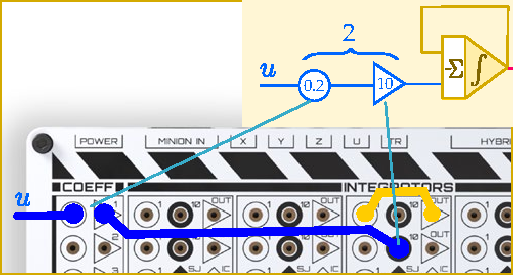
\includegraphics[width=.8\textwidth]{figuras/ejemplo}
%	\caption{Implementación de un coeficiente mayor a la unidad.}
%	\label{fig:ejemplo}
%\end{figure}
%
%Como se ilustra en la figura~\ref{fig:ejemplo}, podemos implementar este coeficiente en el \that si ajustamos $0.225$ en el potenciometro correspondiente y al mismo tiempo lo introducimos multiplicado por 10 en el integrador. Así, el valor equivalente que estamos colocando a la entrada del integrador es:
%\[a_{11}=10 \times 0.225=2.25\]
%
%\item Verifique que la nueva frecuencia de corte es $200$ Hz, variando apropiadamente la frecuencia del generador.
%
%\item Ajuste una onda \tt{SWEEP} y 	verifique el funcionamiento del filtro. 
%\end{enumerate}
%
%\newpage
%
%\section{Estabilidad de un sistema realimentado y test de estabilidad de Routh- Hurwitz}
%
%En esta última sección vamos a analizar la estabilidad del sistema realimentado de la figura~\ref{fig:realimentado}:
%%
%\begin{figure}[h!]
%	\centering
%	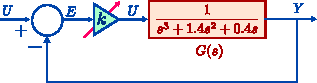
\includegraphics[width=.65\textwidth]{figuras/realimentado}
%	\caption{Implementación de un coeficiente mayor a la unidad.}
%	\label{fig:realimentado}
%\end{figure}
%
%Este sistema tiene función de transferencia de lazo cerrado $H_r(s)$, dada por:
%\begin{align}
%H_r(s) = \dfrac{Y(s)}{U(s)} &= \dfrac{kG(s)}{1+kG(s)}\nonumber\\
%	   &= \dfrac{k}{s^3+1.4s^2+0.4s+k}
%	   \label{equ:realimentado}
%\end{align}
%
%
%
%Queremos analizar experimentalmente la estabilidad de $H_r(s)$  para variaciones del parámetro $k$ en que $0 \leq k \leq 1$, usando el \that
%
%\newpage
%\subsection{Implementación}
%
%Note que la función $G(s)$ en el lazo realimentado la podemos expresar como:
%
%\begin{align}
%	G(s)&=G_1(s) \times G_2(s) \times G_3(s) \nonumber\\
%	&=\dfrac{1}{s+1} \times \dfrac{1}{s+0.4} \times \dfrac{1}{s}.
%\end{align}
%
% Y cada bloque de primer orden lo podemos realizar como se ilustra en la figura~\ref{fig:analoghurwitz}
% %
%\begin{figure}[h!]
%	\centering
%	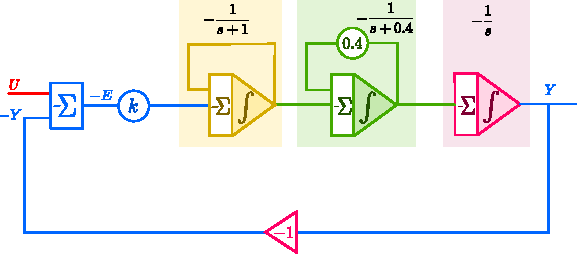
\includegraphics[width=.9\textwidth]{figuras/analoghurwitz}
%	\caption{Implementación de computador analógico.}
%	\label{fig:analoghurwitz}
%\end{figure}
%
%
%\subsection{Pasos de implementación}
%
%\begin{enumerate}[label=\alph*)]
%		
%	\item Discuta con su compañero, porque los bloques en color de la figura~\ref{fig:analoghurwitz} implementan a $G_1$, $G_2$ y $G_3$.
%	
%	\item Desconecte todos los cables del \that, incluyendo el conector RCA y el generador de onda.
%	
%	\item Realice nuevamente el generador de onda del \that~ de  la sección~\ref{sec:cuadrada} 
%	
%	\item Implemente cuidadosamente en el \that~ el diagrama de la figura \ref{fig:analoghurwitz}. Use los bloques apropiados.
%	\item Conecte el canal 1 y el canal 2 a la entrada $U$ y la salida $Y$ del sistema como en la figura~\ref{fig:analog2orderthat}.
%	
%	\item Ponga el \tt{THAT} en modo \tt{REPF}.
%	
%	\item Varie el coeficiente correspondiente a $k$ y determine por la respuesta percibida en el osciloscopio, el punto en que el sistema cambia de estable a inestable. Registre este valor pasando el \tt{THAT} al modo \tt{COEFF}.
%	
%	\item Use el criterio de Routh - Hurwitz  para obtener matematicamente el rango de estabilidad del sistema realimentado de la ecuación~\eqref{equ:realimentado} (puede usar gemini u otra). Compare con lo obtenido experimentalmente.
%\end{enumerate}
%\section{solucion}
%\begin{tabular}{|c|c|c|c|c|}
%	\hline
%	& E con $\zeta =0.3$ & T con $\zeta = 0.3$  & E $SP =10$   & T  $SP =10$ \\
%	\hline
%$t_r$	& 2.7 &  2.65 &  &  \\
%	\hline
%$SP$	& 38.3 & 37.23 &  &  \\
%\hline
%$t_{ee}$	&  &  &  &  \\
%\hline
%	\hline
%\end{tabular}
\end{document}
